\documentclass[border={5pt 5pt 5pt 5pt}]{standalone}
\usepackage{tikz}
\usetikzlibrary{bayesnet}
\usetikzlibrary{arrows}
\usepackage{color}
\usepackage{graphicx}
\usepackage{caption}
\usepackage{subcaption}

\begin{document}
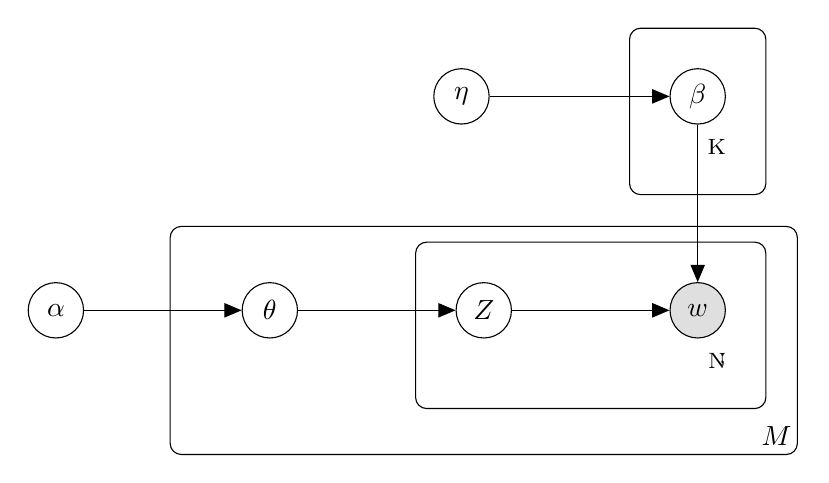
\begin{tikzpicture}

    %nodes
    \node[obs] (w) {$w$};
    \node[latent, above=of w, xshift=-3cm, yshift=1cm] (eta) {$\eta$};
    \node[latent, above=of w, yshift=1cm] (beta) {$\beta$};
    \node[latent, left=of w, xshift=-1cm] (Z) {$Z$};
    \node[latent, left=of Z, xshift=-1cm] (theta) {$\theta$};
    \node[latent, left=of theta, xshift=-1cm] (alpha) {$\alpha$};
    \node [below=of w, xshift=1cm] {$M$};
    
    % edges
    \edge {eta} {beta}  
    \edge {beta} {w}
    \edge {alpha} {theta}  
    \edge {theta} {Z}  
    \edge {Z} {w}  
    
    % plate
    \plate [inner sep=0.5cm, xshift=.0cm, yshift=0.0cm] {plate1} {(beta)} {K}; %
    \plate [inner sep=0.9cm, xshift=.0cm, yshift=-0.2cm] {plate2} {(theta)(Z)(w)}; %
    \plate [inner sep=0.5cm, xshift=.0cm, yshift=0.0cm] {plate3} {(Z)(w)} {N}; %
    
    % \node[latent,above=of x,xshift=-1cm] (mu) {$\mu$}; %
    % \node[latent,above=of x] (r) {$r$}; %
    % \node[latent,above=of x,xshift=1cm] (sigma) {$\sigma$}; %
    % plate
    % \plate [inner sep=.3cm,xshift=.02cm,yshift=.2cm] {plate1} {(x)} {$i$ data}; %
    % edges
    % \edge {r,sigma,mu} {x}  
\end{tikzpicture}
\end{document}